\chapter{Natural Gas Flow}
\label{chap:fund_NGF}

The steady-state Natural Gas Flow (NGF) problem for transmission networks aims to find the value for a set of state-variables that satisfy the flow balance in all nodes. We show how the NGF can be derived in a similar way as the Power Flow (PF) problem is introduced for power systems. In  particular, a set of nonlinear equations must be solved where the definition of the state-variables depends on the selected models for all the elements of the system. In this section, we derive the NGF problem and introduce the modeling for the main elements considered in \mpng{}: nodes, wells, pipelines, compressors, and storage units.

\section{Modeling}
\label{sec:gas_modeling}

An exact description of the natural gas flow in transmission networks requires applying the laws of fluid mechanics and thermodynamics \cite{Osiadacz2001}. Complex analyzes provide an accurate description for variables such as temperature, pressure, flow, adiabatic head, among others, for all time instants. However, as the primary concern of \matpower{} (and so does \mpng{}) is the system operation in steady-state, we define some models to describe the main elements of the default natural gas network, as explained below. 

\subsection{Nodes}
\label{subsec:nodes}

By definition, a node is the location of a natural gas system where one or more elements are connected. Users are commonly associated with a node where a stratified demand is modeled as different market segments that get different priorities. Figure \ref{fig:node} shows the $i$-th node of a gas network with some traditional markets connected to form the nodal demand $f_{dem}=\sum_{j} f_{\text{dem}_j}$. The primary variable related to a node is pressure $p_i$.

\begin{figure}[!ht]
	\centering
	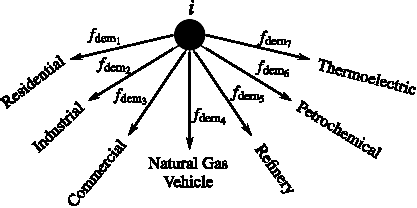
\includegraphics[scale=1.2]{Figures/Node}
	\caption{A natural gas node and some traditional markets.}	
	\label{fig:node}
\end{figure}


\subsection{Wells}
\label{subsec:wells}

Natural gas is extracted from deep underground and injected into the system in wells. Depending on the well capacity, injection could be made either at constant pressure, where a control system regulates the amount of gas flow such that pressure behaves constant, or at constant flow, where pressure is adjusted such that injected flow remains constant. Figure \ref{fig:well} shows a well connected to the $i$-th node whose operation depends on two principal variables, the injected gas flow $f_{inj}^w$, and the nodal pressure $p_i$.

\begin{figure}[!ht]
	\centering
	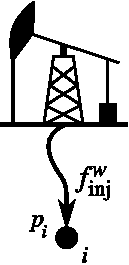
\includegraphics[scale=0.9]{Figures/Well}
	\caption{A natural gas well.}	
	\label{fig:well}
\end{figure}

\subsection{Pipelines}
\label{subsec:pipelines}

In general, the flow of gas through pipes is studied using the energy equation of fluid mechanics~\cite{Banda2006}. However, in practice, the relationship between the gas flow in the pipe and the upstream and downstream pressures can be described by various equations. The Weymouth's general flow equation is the frequent option in gas industry applications to model the steady-state flow in pipes in transmission networks~\cite{Woldeyohannes2011}. Figure \ref{fig:pipeline} shows a pipeline $o$ whose gas flow from the node $i$ to the node $j$ is represented by $f_{ij}^o$. The Weymouth's equations states the relationship between $f_{ij}^o$, $p_i$, and $p_j$ in the following form:

\begin{equation}
	\label{eq:Weymouth_eq1}
	\text{sgn}(f_{ij}^o)(f_{ij}^o)^2 = K_{ij}(p_i^2-p_j^2). 
	\vspace{0.3cm}
\end{equation}

\begin{figure}[!ht]
	\centering
	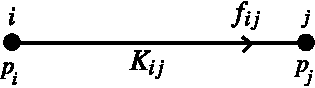
\includegraphics[scale=1]{Figures/Pipeline}
	\caption{A natural gas pipeline.}	
	\label{fig:pipeline}
\end{figure}

In Equation \ref{eq:Kij}, $\text{sgn}(\cdot)$ represents the sign function, and $K_{ij}$ is the  Weymouth constant\footnote{Measured in Million Standard Cubic Feet per Day (MMSCFD) over psia. Different expressions for $K_{ij}$ can be derived depending on the parameters used in the flow equations. See \cite{Woldeyohannes2011} and reference therein for details.} of the pipeline defined in terms of the pipe length and diameter as below~\cite{Wolf2000}:

\begin{equation}
	\label{eq:Kij}
	K_{ij} = \sqrt{5.695756510\times 10^{-13}\:\frac{D^5}{\lambda Z T L\delta}}\quad \left[\frac{\text{MSCFD}}{\text{psia}}\right],
	\vspace{0.3cm}
\end{equation}

where: 

\begin{equation}
	\label{eq:lambda_Kij}
	\frac{1}{\lambda} = \left[2\log \left(\frac{3.7D}{\varepsilon}\right)\right]^2,
	\vspace{0.3cm}
\end{equation}

with:

\begin{labeling}{alligator}
	\item [$\qquad \qquad  D$]  \hspace{0.8cm} Diameter [in].
	\item [$\qquad \qquad  L$]  \hspace{0.8cm} Length [km]. 
	\item [$\qquad \qquad  T$] \hspace{0.8cm} Gas temperature [K].
	\item [$\qquad \qquad  \varepsilon$] \hspace{0.8cm} Absolute rugosity [mm].
	\item [$\qquad \qquad  \delta$] \hspace{0.8cm} Gas density relative to air [-].
	\item [$\qquad \qquad  Z$] \hspace{0.8cm} Gas compressibility factor [-].
\end{labeling}

For mathematical convenience, we rewrite Equation \ref{eq:Weymouth_eq1} as follows:

\begin{equation}
	\label{eq:Wymouth_eq_2}
	f_{ij}^o = K_{ij} \;\text{sgn}(\pi_i - \pi_j)\sqrt{|\pi_i-\pi_j|},
	\vspace{0.3cm}
\end{equation}

\noindent where $\pi=p^2$ is defined as the quadratic pressure. 

As seen, the gas flow through a pipeline is a nonlinear function of the quadratic pressures of the initial and final nodes, that is, $f_{ij}^o=g(\pi_i,\pi_j)$. 

\subsection{Compressors}
\label{subsec:compressors}
As seen in Equation \ref{eq:Wymouth_eq_2}, there exists a downstream pressure drop when transporting large flows through pipes caused by energy losses. Analogous to the transformer in power systems, compressors are installed in the gas network to compensate pressure drops. Figure \ref{fig:compressor} shows a compressor $c$ that increases the discharge pressure $p_j$ with respect to the suction pressure $p_i$ by compressing gas in a way that a flow $f_{ij}^c$ passes through it. The power demanded by the compressor, $\psi_c$, states the relationship between the flow and the suction and discharge pressures in the following way~\cite{Shabanpour2016}:

\begin{equation}
	\label{eq:comp_flow}
	f_{ij}^c = \frac{\psi_c}{B_c \left[\left(\frac{\pi_j}{\pi_i}\right)^{\frac{Z_c}{2}}-1\right]},
	\vspace{0.3cm}
\end{equation}

where $B_c$ is the compressor constant that describes its construction features, $Z_c$ is the compressibility factor, and $\pi=p^2$ is again the quadratic pressure.

\begin{figure}[!ht]
	\centering
	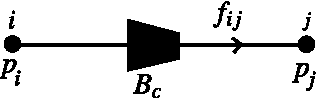
\includegraphics[scale=0.9]{Figures/Compressor}
	\caption{A natural gas compressor.}	
	\label{fig:compressor}
\end{figure}

Moreover, the compressor ratio, $\beta_c$, is defined as below:

\begin{equation}
	\label{eq:comp_ratio}
	\beta_c = \frac{\pi_j}{\pi_i}, \quad \beta_c\geq 1.
	\vspace{0.3cm}
\end{equation}

In general, there exists two types of compressors: the power-driven compressors, whose demanded energy is supplied from the power system, and the gas-driven compressors, that requires additional gas to operate. In the latter, the additional gas demanded at the suction node, $\phi_c$, can be expressed as a quadratic function of the power as~\cite{Chen2017}:

\begin{equation}
	\label{eq:f_cons_gas_comp}
	\phi_c = x+y\psi_c+z\psi_c^2, 
	\vspace{0.3cm}
\end{equation}

where $x,y,z \in \Real$.

Notice that the gas flow through a compressor (and so does the consumed flow for a gas-driven compressor) is a function of the consumed power and the quadratic suction and discharge pressures, that is, $f_{ij}^c=h(\pi_i,\pi_j,\psi_c)$. 

\subsection{Storage Units}
\label{subsec:sto_units}

The possibility of storing natural gas provides flexibility with regards to production and transportation decisions~\cite{Midthun2007}. A storage unit is a reservoir that allows both storing and injection of gas. Figure \ref{fig:storage} shows a storage unit located at node $i$ with an associated gas flow $f_s$ that could be either an \textit{outflow} in the case of injection to the system or an \textit{inflow} in the case of storing operation. Then, in a node with a specific demand and injection, the (known) value of $f_s$ could be added to the nodal demand when it is a storage inflow or could be summed to the injection flow of a constant-flow well when it is a storage outflow.

\begin{figure}[!ht]
	\centering
	
\includegraphics[scale=1]{Figures/Storage_unit}
	\caption{A natural gas storage unit.}	
	\label{fig:storage}
\end{figure}

\section{Deriving the Natural Gas Flow Problem}
\label{sec:NGF_problem}

Let us consider the transmission natural gas network shown in Figure \ref{fig:nodal_balance}. According to the principle of conservation of mass, the balance equation applied to the node $i$ states:

\begin{equation}
	\label{eq:balance_eq}
	f_{inj} - f_{dem} \pm f_s = \sum_{\substack{j=1 \\ j \neq i}}^{m} f_{ij},
\end{equation}

where $f_{dem}$ is the known demand flow, $f_s$ is either the  inflow (negative) or outflow (positive) of the storage unit, and $f_{inj}$ is the injected flow of the well. 

\begin{figure}[!ht]
	\centering
	
\includegraphics[scale=0.95]{Figures/Gas_flow_problem}
	\caption{Nodal balance in a transmission natural gas network.}	
	\label{fig:nodal_balance}
\end{figure}

Notice in equation \ref{eq:balance_eq} that the left hand side is a known value if injection is produced by a constant-flow well. However, for a constant-pressure well, the value of $f_{iny}$ must be determined. In turn, the algebraic sum of the right hand side depends on the nature of the elements connected between nodes $i$ and $j$ such that $f_{ij}$ takes the form of $f_{ij}^o$ or $f_{ij}^c$, according to Equations \ref{eq:Wymouth_eq_2} and \ref{eq:comp_flow}, for a pipeline or a compressor, respectively. Moreover, for a gas-driven compressor, the additional gas consumption $\phi_c$ must be considered as an outflow in Equation \ref{eq:balance_eq} if node $i$ matches the suction node for compressor $c$.

%such that $f_{ij}$ is $g(\pi_i,\pi_j)$, $h(\pi_i,\pi_j,\psi_c)$, or $h(\pi_i,\pi_j,\psi_c)+\phi_c(\psi_c)$ for a pipeline, a power-driven compressor, and a gas-driven-compressor, respectively.

As a consequence, we can rewrite the balance equation applied at node $i$ in a functional form as follows:

\begin{equation}
	\label{eq:balance_eq_funtional}
	\mathbb{F}_i\left(\pi,\psi_c,f_{iny}^{w}\right) = 0.
	\vspace{0.3cm}
\end{equation}

In practice, for a given gas network with $n_n$ nodes, $n_c$ compressors, and $n_{w_p}$ constant-pressure wells, the application of the balance equation for all nodes will produce a set of $n_n$ nonlinear equations with a number of $(n_n-n_{w_p})+n_c+n_{w_p} = n_n+n_c$ unknown variables. To get a squared system with the same number of equations and variables, the $n_c$ missing equations are obtained from the compressor ratios of all compressors. Then, the NGF problem can be formulated as follows:

\begin{equation}
	\label{eq:F_i=0}
	\mathbb{F}_i\left(\pi,\psi_c,f_{iny}^{w}\right) = 0, \quad \forall i\in\mathcal{N}, c\in\mathcal{C}; w\in\mathcal{W}_p, 	
\end{equation}

\begin{equation}
	\label{eq:R_c=0}
	\beta_c = \frac{\pi_j}{\pi_i}, \quad \forall c\in\mathcal{C}, \;  i,j\in\mathcal{N},
	\vspace{0.3cm}
\end{equation}

where

\begin{labeling}{alligator}
	\item [$\qquad \qquad  \mathcal{N}$]  \hspace{0.85cm} Set of gas nodes, $|\mathcal{N}|=n_n$.
	\item [$\qquad \qquad  \mathcal{C}$]  \hspace{1cm} Set of compressors, $|\mathcal{C}|=n_c$. 
	\item [$\qquad \qquad  \mathcal{W}_p$] \hspace{0.65cm} Set of constant-pressure wells, $|\mathcal{W}_p|=n_{w_p}$.	
\end{labeling}



